\documentclass[10pt,a4paper]{amsart}
\usepackage{amsmath,amssymb,amsthm,graphicx}
\usepackage{amsmath,amssymb,amsthm,xfrac,xspace,hyperref,graphicx,comment}
\excludecomment{DefTralics}
\providecommand{\dpl}{\displaystyle}
\providecommand{\backmatter}{}
\providecommand{\loccit}{\emph{loc. cit.}}

\providecommand{\bibliofont}{\small}
\newcommand{\ie}{i.e.,\xspace}
\newcommand{\eg}{e.g.,\xspace}
\newcommand{\etc}{etc.\xspace}
\newcommand{\cf}{cf.\xspace}
\newcommand{\resp}{resp.\xspace}
\providecommand{\smaller}{\small}
\newcommand{\Subsection}{\subsection}
\newcommand{\Subsubsection}{\subsubsection}
\newcommand{\skpt}{\smallskip}
\emergencystretch=3em
\numberwithin{equation}{section}
\usepackage[scr=rsfs,cal=euler]{mathalfa}
\let\mathds\mathbb
\let\epsilon\varepsilon
\newcommand{\Changel}{\mathcode`l="7160}
\newcommand{\Changelback}{\mathcode`l="716C}
\newcommand{\NoChangel}[1]{%
\expandafter\let\csname old\string#1\endcsname=#1
\let#1=\relax
\newcommand{#1}{\mathcode`l="716C\csname old\string#1\endcsname\mathcode`l="7160 }%
}

\NoChangel{\log}
\NoChangel{\ln}
\NoChangel{\lim}
\NoChangel{\limsup}
\NoChangel{\liminf}
\NoChangel{\varlimsup}
\NoChangel{\varliminf}
\NoChangel{\varinjlim}
\NoChangel{\varprojlim}

\newenvironment{enumeratei}
{\bgroup\def\theenumi{\roman{enumi}}\def\theenumii{\arabic{enumii}}\begin{enumerate}}
{\end{enumerate}\egroup}
\newcommand{\Psfrac}[2]{(\sfrac{#1}{#2})}
\newcommand{\psfrac}[2]{\sfrac{(#1)}{#2}}
\newcommand{\spfrac}[2]{\sfrac{#1}{(#2)}}
\newcommand\mto{\mathchoice{\longmapsto}{\mapsto}{\mapsto}{\mapsto}}
\newcommand\hto{\mathrel{\lhook\joinrel\to}}

\usepackage{graphicx}

\newtheorem{thm}{Theorem}[section]
\newtheorem{cor}[thm]{Corollary}
\newtheorem{lem}[thm]{Lemma}
\newtheorem{prop}[thm]{Proposition}
\newtheorem{quest}{Question}[section]
\newtheorem{conj}{Conjecture}[section]
\newtheorem{maintheorem}{Theorem}
\theoremstyle{definition}
\newtheorem{rem}[thm]{Remark}
\newtheorem{exm}[thm]{Example}
\newtheorem{ass}[thm]{Assumption}
\renewcommand*{\themaintheorem}{\Alph{maintheorem}}

\DeclareMathOperator{\area}{area}
\DeclareMathOperator{\lcm}{lcm}
\DeclareMathOperator{\const}{const}
\DeclareMathOperator{\Cal}{Cal}
\DeclareMathOperator{\Flux}{\mathrm{Flux}}
\newcommand{\id}{\mathrm{id}}
\newcommand{\Ham}{\mathrm{Ham}}
\newcommand{\std}{\mathrm{std}}
\newcommand{\vol}{\mathrm{vol}}
\newcommand{\fix}{\mathrm{fix}}
\newcommand{\pr}{\mathrm{pr}}
\newcommand{\Tan}{\mathrm{T}}
\newcommand{\N}{\mathds{N}}
\newcommand{\Z}{\mathds{Z}}
\newcommand{\R}{\mathds{R}}
\newcommand{\CC}{\mathds{C}}\let\C\CC
\newcommand{\UU}{\mathcal{U}}
\newcommand{\VV}{\mathcal{V}}

\let\eul e
\let\diff d
\title{A connected global surface of section bounded by any chosen Besse Reeb orbit}
\author{Alberto Abbondandolo, Christian Lange, Marco Mazzucchelli}
\date{doi:10.5802/jep.195; CC BY 4.0}
\makeatletter
\newlabel{mt:surface}{{source: mt:surface}{}{}{}{}}
\newlabel{t:main}{{source: t:main}{}{}{}{}}
\makeatother
\begin{document}
\noindent\textit{Reference locators: references to unnumbered external source sections retain their original author labels; complete source files accompany this item.}\par
\maketitle
\noindent\textit{Editorial note.} Source1008 overstates uniqueness of the dual pair for(alpha,beta)=(1,0): determinant1 requires beta-prime=1, while alpha-prime is free. The displayed(0,1) is a valid choice used for the regular-orbit model. The original wording remains.\par\medskip
\noindent\textit{Editorial note.} Source995 writes B\_i when defining the j-th solid torus Y\_j; surrounding993/997 and the subsequent gluing identify the disk as B\_j. The original formula remains unchanged.\par\medskip
\noindent\textit{Editorial note.} The auxiliary local setup1070 permits negative p\_0, for which its later positive-intersection/orientation assertion is not valid in general. The counted theorem1092 and its construction1125/1131 explicitly require and produce p\_0>0. Only this positive-cover branch is used and endorsed in the current problem; the printed broader auxiliary wording is retained and disclosed.\par\medskip
\noindent\textit{Editorial note.} The coordinate projection(z,s)->z in995 is not the orbit quotient for the twisted circle action1025 when alpha\_j-prime is nonzero. The classical Seifert orbit quotient is allowed as background, but those two maps must not be identified. The actual positive-cover proof uses the coordinate solid-torus neighborhoods, boundary bases, explicit action and horizontal caps; the exterior Y\_0 has the genuine product projection. The original pi formulas are retained: no replacement pi or new gluing proof is inserted.\par\medskip
\noindent\textit{Editorial note.} Panel(a) of the original figure labels the large cut base region with an intersection sign. The author explicitly defines B\_0-prime in1157 as B\_0 minus the connecting rectangles, and that cut region is used in the subsequent sheet construction. The original figure is retained.\par\medskip
\noindent\textit{Allowed standard prerequisites (editorial).}\begin{itemize}
\item Classical Seifert surgery description of locally free circle actions on oriented three-manifolds. The classical Seifert orbit space, explicit locally free circle action and surgery/gluing conventions are allowed background, not a global-section existence theorem. Distinguish the true orbit quotient from the coordinate projection(z,s)->z printed995: the latter is not invariant under the twisted action1025. The proof uses coordinate solid tori, their boundary bases and the stated action; on the free exterior Y\_0 the displayed product projection is the orbit quotient. No replacement formula for the author pi is inserted or assumed.
\item Besse Reeb periodicity and negative rational Euler number. Provides the locally free action and e(Y)<0; the positive covering coefficients and global surface are still constructed.
\item Equivariant local contact normal form via Moser method. The tubular form1065 is permitted; local section slope choices and all gluing remain obligations.
\item Elementary oriented-surface cut-and-paste, torus homology and Bezout/lcm arithmetic. No global-section existence theorem from Albach–Geiges is supplied as a prerequisite.
\end{itemize}\medskip
The aim of this paper is to prove some sharp inequalities involving the periods of closed orbits of Reeb flows on $3$-manifolds and the contact volume.
Let $Y$ be a closed, connected, orientable $3$-manifold. We recall that a one-form $\lambda$ on $Y$ is called a contact form when $\lambda\wedge d\lambda$ is nowhere vanishing. The contact form $\lambda$ induces a vector field $R_{\lambda}$, which is called Reeb vector field of $\lambda$, by the identities $R_{\lambda} \,\lrcorner\, \diff\lambda = 0$ and $R_{\lambda} \,\lrcorner\, \lambda=1$.
The flow of $R_{\lambda}$ is called the Reeb flow, and we will denote it by $\phi_{\lambda}^t$. It preserves the contact form $\lambda$, and in particular the volume form $\lambda\wedge d\lambda$. Reeb flows are also called contact flows in the literature. Reeb flows on $3$-manifolds constitute a special class of volume preserving flows with the remarkable feature of always having closed orbits: the Weinstein conjectures postulates that Reeb flows on arbitrary closed contact manifolds admit closed orbits, and this conjecture has been confirmed in dimension $3$ by Taubes, see \cite{Taubes:2007wi}.

Borrowing once more the terminology from Riemannian geometry, a contact form~$\lambda$ on~$Y$ is called Besse if all its Reeb orbits are closed. Here, different Reeb orbits are not required to have the same minimal period, and therefore Besse contact forms constitute a larger class than Zoll forms. Thanks to a theorem of Wadsley \cite{Wadsley:1975sp} or, in the special case of dimension $3$, an earlier theorem of Epstein \cite{Epstein:1972}, Besse Reeb flows are periodic (see also \cite{Sullivan:1978}). In our case, since $Y$ has dimension $3$, Epstein's theorem implies that all Reeb orbits of the Besse contact form $\lambda$ have the same minimal period $T$ except for finitely many ones, whose minimal period divides~$T$. The orbits of the first kind are called regular, whereas the finitely many exceptional orbits with smaller minimal period are called singular.

\subsection{Global surfaces of section}
\label{s:sos_def}
In this paper, a global surface of section for a contact form $\lambda$ on a $3$-manifold $Y$ is a smooth map $\iota:\Sigma\to Y$, where $\Sigma$ is an oriented connected compact surface with non-empty and possibly disconnected boundary, with the following properties:
\begin{itemize}

\item \textit{$($Boundary$\,)$} The restriction $\iota|_{\partial\Sigma}$ is an immersion positively tangent to the Reeb vector field $R_{\lambda}$. Namely, with the orientation on the boundary $\partial\Sigma$ induced by the one of $\Sigma$,
the restriction of $\iota$ to any connected component of $\partial\Sigma$ is an orientation preserving covering map of a closed Reeb orbit of $(Y,\lambda)$.\vspace{2pt}

\item \textit{$($Transversality$\,)$} The restriction $\iota|_{\mathrm{int}(\Sigma)}$ is an embedding into $Y\setminus\iota(\partial\Sigma)$ transverse to the Reeb vector field $R_\lambda$.
In particular, the $2$-form $\iota^*\diff\lambda$ is nowhere vanishing on $\mathrm{int}(\Sigma)$, and we assume that it is a positive area form on the oriented surface $\mathrm{int}(\Sigma)$.\vspace{2pt}

\item \textit{$($Globality$\,)$} For each point $z\in Y$, the Reeb orbit $t\mto\phi_\lambda^t(z)$ intersects $\Sigma$ in both positive and negative time.

\end{itemize}
We stress that, in the literature, the notion of global surface of section may be slightly different than the one given here: for instance, the map $\iota:\Sigma\to Y$ may be required to be an embedding, or the restriction of $\iota$ to some connected component of $\Sigma$ may be allowed to be an orientation reversing covering map of a closed Reeb orbit.

\Subsection{The surgery description of a Besse contact form on a $3$-manifold}
\label{s:surgery}

The proof of Theorem~\ref{t:main} will require suitable surfaces of section for the Reeb flows of contact forms sufficiently $C^3$-close to a Besse one. As a preliminary step, in the next subsection we shall construct global surfaces of sections for the Reeb flow of Besse contact $3$-manifolds. It will be useful to employ the surgery description of Besse contact $3$-manifolds as Seifert fibered spaces, which we now recall. We refer the reader to, e.g., \cite{Orlik:1972ts,Jankins:1983zm} for more details.

A Seifert fibration $\pi:Y\to B$, in the generality that we need for the study of Besse contact $3$-manifolds, is defined up to a suitable notion of isomorphism by a genus and $k\geq1$ pairs of coprime integers $(\alpha_1,\beta_1),\dots,(\alpha_k,\beta_k)\in\N\times\Z$. Here, $\N$ denotes the set of positive integers and the coprimeness assumption implies that $\alpha_j=1$ if $\beta_j=0$. We denote by $B_0$ an oriented compact connected surface of the given genus with $k$ boundary components. We write its oriented boundary as $\partial B_0=\partial_1 B_0\cup\dots\cup\partial_{k} B_0$, where each $\partial_j B_0$ is a connected component oriented as the boundary of $B_0$. Over $B_0$, we consider the trivial $S^1$-bundle
\[
\pi:Y_0:=B_0\times S^1\to B_0,\qquad \pi(z,t)=z,
\]
with its associated free $S^1$-action
\[
t\cdot(z,s)=(z,s+t),\qquad \forall t\in S^1,\ (z,s)\in Y_0.
\]
Here and elsewhere in the paper, $S^1=\R/\Z$.
Next, we consider $k$ disjoint copies $B_j\subset \C$, $j=1,\dots,k$ of the disk of some radius $\rho>0$ centered at the origin, and the solid tori together with their base projections
\[
\pi:Y_j:=B_i\times S^1\to B_j,\qquad \pi(z,t)=z.
\]
By the Bézout identity, we can find pairs of coprime integers $(\alpha_j',\beta_j')\in \Z\times \Z$ such that
\begin{equation}
\label{e:dual_Seifert_pair}
\det
\begin{pmatrix}
\alpha_j & \alpha_j' \\
\beta_j & \beta_j'
\end{pmatrix}=1,
\qquad
\forall j=1,\dots,k.
\end{equation}
The pair $(\alpha_j',\beta_j')$ is not uniquely determined by $(\alpha_j,\beta_j)$ (except if $(\alpha_j,\beta_j)=(1,0)$, in which we necessarily have $(\alpha_j',\beta_j') = (0,1)$). We introduce the oriented curves\Changel
\begin{align*}
m_j&=\partial B_j\times\{*\}\subset \partial Y_j,
&
l_j&=\{*\}\times S^1 \subset \partial Y_j,
\\
h_j&=\{*\}\times S^1\subset \partial_j B_0\times S^1 \subset\partial Y_0,
&
f_j&=-\partial_j B_0\times\{*\} \subset\partial Y_0.
\end{align*}
Here, we used the symbol $*$ to denote an arbitrary point of a space. We glue $Y_0,Y_1,\dots,Y_k$ along their boundaries by identifying
\[
m_j\equiv\alpha_jf_j+\beta_j h_j,\qquad l_j\equiv\alpha_j'f_j+\beta_j'h_j,\qquad \forall j=1,\dots,k
\]
and denote by $Y$ the resulting closed $3$-manifold. Here, we mean that $m_j\subset\partial Y_j$ is identified with an oriented embedded circle in $\partial_j Y_0$ that is homologous to $\alpha_j[f_j]+\beta_j[h_j]$, and analogously for $l_j$.
The free $S^1$-action on $Y_0$ extends to an $S^1$-action on the whole $Y$, which on the solid tori $Y_j$ has the form\Changelback
\[
t\cdot(z,s)=\big(z e^{-2\pi\alpha_j't i},s+\alpha_j t\big),
\qquad
\forall t\in S^1,\ (z,s)\in Y_j.
\]
If $\alpha_j>1$, the $S^1$-action is not free on the orbit
\[
\gamma_j:=\{0\}\times S^1\subset Y_j,
\]
and in this case we call such an orbit singular. All those $S^1$-orbits that are not singular are called regular.
The surfaces $B_j$ are glued accordingly to form a closed surface $B$. The maps $\pi$ are glued as well, and the obtained $\pi:Y\to B$ is the quotient projection of the $S^1$-action on $Y$.
We can always assume without loss of generality that the number of Seifert pairs $(\alpha_j,\beta_j)$ is $k\geq2$; indeed, adding the trivial Seifert pair $(1,0)$ does not affect the Seifert fibration.

The locally free $S^1$-action that is induced by a Besse Reeb flow on $Y$ can be seen as the $S^1$-action on the total space of a Seifert fibration $\pi:Y\to B$ as above. In this case, the Euler number
\[
\eul(Y):=-\frac{\beta_1}{\alpha_1}-\dots-\frac{\beta_k}{\alpha_k}
\]
is negative, as shown in \cite{Lisca:2004oz} (see also \cite[Th.\,1.4]{Kegel:2021vo}).

\Subsection{A Global surface of section for a Besse contact form on a $3$-manifold}
\label{s:sos_Besse}
The existence of global surfaces of section in Seifert spaces was thoroughly investigated by Albach-Geiges \cite{Albach:2021wi}. In this subsection, we prove a statement which may be of independent interest (Theorem~\ref{t:sos_Besse}) asserting that on a Besse contact $3$-manifold any given closed Reeb orbit is the (multiply covered) boundary of a surface of section as defined in Section~\ref{s:sos_def}

Let $(Y,\lambda_0)$ be a Besse contact $3$-manifold whose Reeb orbits have minimal common period~$1$, and $\gamma_1$ be an arbitrary closed Reeb orbit. The Reeb flow $\phi_{\lambda_0}^t$ defines a locally free $S^1$-action on $Y$. We can see this action as the $S^1$-action of a Seifert fibered structure which we describe with the same notation of the previous subsection: in particular, for each $j=1,\dots,k$, we denote by $\gamma_j$ the closed Reeb orbit corresponding to the Seifert pair $(\alpha_j,\beta_j)$. Notice in particular that we are assuming without loss of generality that our given $\gamma_1$ is the closed Reeb orbit corresponding to the Seifert pair $(\alpha_1,\beta_1)$. We recall that $\gamma_1$ has minimal period $1/\alpha_1$, and therefore it is a singular orbit if and only if $\alpha_1>1$.

We consider the tubular neighborhood $Y_1\subset Y$ of $\gamma_1$, which was realized as $Y_1\equiv B_1\times S^1$, and under this identification we have $\gamma_1=\{0\}\times S^1\subset Y_1$.
We equip $Y_1$ with the contact form
\[
\lambda_0' = \frac{1}{\alpha_1}\,r^2\diff\theta + \frac{1}{\alpha_1}\big(1+2\pi\Psfrac{\alpha'_1}{\alpha_1}r^2\big) \diff s,
\]
where $(r,\theta)$ are polar coordinates on the disk $B_1$, and $s\in S^1=\R/\Z$.
The associated Reeb vector field is given by
\[
R_{\lambda_0'} = -2\pi\alpha_1'\partial_\theta + \alpha_1\partial_s=R_{\lambda_0}|_{Y_1},
\]
and therefore the associated Reeb flow agrees with the Seifert $S^1$-action
\[
\phi_{\lambda_0'}^t(z,s)=\phi_{\lambda_0}^t(z,s)=t\cdot(z,s)=\big(z e^{-2\pi\alpha_1't i},s+\alpha_1 t\big).
\]
Up to pulling back $\lambda_0$ by an $S^1$-equivariant diffeomorphism, we can assume that
\[
\lambda_0|_{Y_1}=\lambda_0'=\frac{1}{\alpha_1}\,r^2\diff\theta + \frac{1}{\alpha_1}\big(1+2\pi\Psfrac{\alpha'_1}{\alpha_1}r^2\big) \diff s.
\]
This can be obtained by means of a Moser's trick, see \cite[Lem.\,4.5]{Cristofaro-Gardiner:2020aa}.
Notice that every orbit of the Reeb flow $\phi_{\lambda_0}^t$ on $Y_1$ has minimal period $1$, except possibly $\gamma_1=\{0\}\times S^1$ that has minimal period $1/\alpha_1$ (the case in which $\gamma_1$ is regular is allowed, and corresponds to the Seifert invariants $(\alpha_1,\beta_1)=(1,0)$).

For any pair of coprime integers $p_0\neq0$ and $q_0$ such that
\begin{equation}
\label{e:transversality}
\frac {q_0}{p_0}< -\frac{\alpha_1'}{\alpha_1},
\end{equation}
and for any $s_0\in S^1$, we introduce the map
\[
\iota:[0,\rho)\times S^1\to B_1\times S^1,\qquad \iota(r,s)=\big( r e^{2\pi (s_0+q_0 s)i},p_0s \big),
\]
which satisfies the following properties:
\begin{itemize}
\item \textit{$($Transversality$\,)$} The restriction $\iota|_{(0,\rho)\times S^1}$ is an embedding transverse to the Reeb vector field $R_{\lambda_0}$, and the image $\iota((0,\rho)\times S^1)$ intersects $-\alpha_1q_0-p_0\alpha_1'>0$ times every Reeb orbit in $Y_1$ other than $\gamma_1$. Therefore, the $2$-form $\iota^*\diff\lambda_0$ is nowhere vanishing on the interior $(0,\rho)\times S^1$, and we employ it to orient the annulus $[0,\rho)\times S^1$.\vspace{2pt}

\item \textit{$($Boundary$\,)$} The restriction $\iota|_{\{0\}\times S^1}$ is an orientation preserving $p_0$-th fold covering map of the closed Reeb orbit $\gamma_1$. Here, the boundary circle $\{0\}\times S^1$ is oriented by means of the $1$-form $\iota^*\lambda_0$.
\end{itemize}
We call $\iota:[0,\rho)\times S^1\to B^2\times S^1$ a $(p_0,q_0)$-local surface of section with boundary on the orbit $\gamma_1$.

We now provide the construction of a suitable global surface of section for the Besse contact $3$-manifold $(Y,\lambda)$ with boundary on the orbit $\gamma_1$. An alternative construction in the special case of a regular orbit in $S^3$ was provided by Albach-Geiges \cite[Ex.\,5.6]{Albach:2021wi}. The next result is a more precise version of Theorem \ref{mt:surface} from the introduction.

\begin{thm}
\label{t:sos_Besse}
Let $(Y,\lambda_0)$ be a Besse contact $3$-manifold with minimal common Reeb period $1$, and $\gamma_1$ be any of its closed Reeb orbits. We denote by $\alpha_1>0$ the integer whose reciprocal $1/\alpha_1$ is the minimal period of $\gamma_1$.
Then, there exist integers $b>0$, $p_0>0$, and $q_0$ with $\gcd(p_0,q_0)=1$, a compact connected oriented surface $\Sigma$ with $b$ boundary components and a global surface of section $\iota:\Sigma\to Y$ for $(Y,\lambda_0)$ satisfying the following properties:
\begin{enumeratei}
\item\label{t:sos_Bessei}
Any connected component $C$ of the boundary $\partial\Sigma$ has a collar neighborhood $A_C\cong[0,\rho)\times S^1$ such that the restriction $\iota|_{A_C}$ is a $(p_0,q_0)$-local surface of section with boundary on the orbit $\gamma_1$. In particular, all boundary components are positively oriented. \vspace{2pt}

\item\label{t:sos_Besseii}
Any regular closed Reeb orbit in $Y\setminus\gamma_1$ intersects the image $\iota(\mathrm{int}(\Sigma))$ in $\alpha$ points, where
\[
\alpha:=- \frac{b\, p_0}{\eul(Y)\, \alpha_1}>0.
\]
Here, $\eul(Y)$ is the Euler number of $(Y,\lambda_0)$.\vspace{2pt}

\item\label{t:sos_Besseiii}
The restriction $\iota|_{\partial\Sigma}$ is a covering map of $\gamma_1$ of degree $b\,p_0$.
\end{enumeratei}
\end{thm}

\begin{figure}
\begin{center}
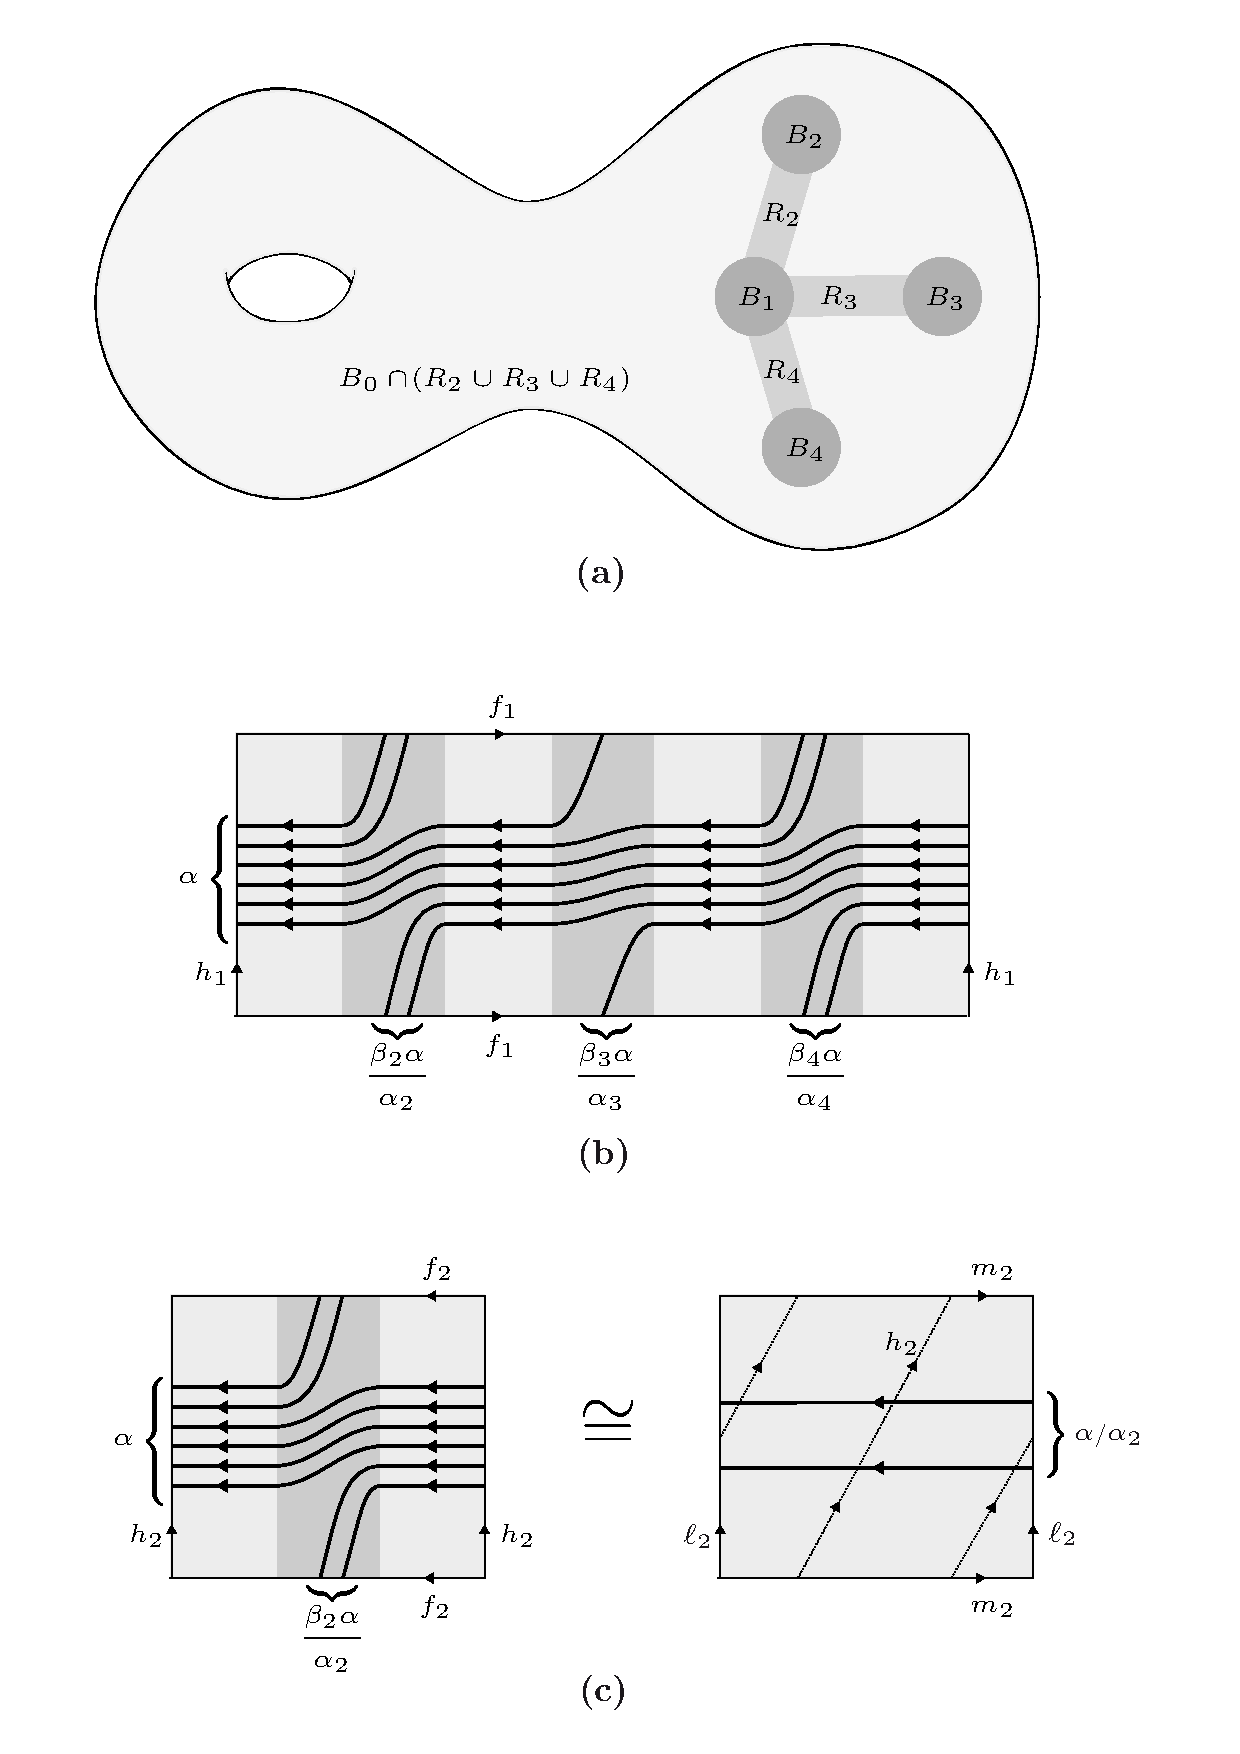
\includegraphics[scale=.46]{abbondandolo-et-al_fig}
\caption{Construction of a global surface of section.}
\label{f:sos}
\end{center}
\end{figure}

\begin{proof}
Let $(\alpha_1,\beta_1),\dots.,(\alpha_k,\beta_k)$ be the Seifert invariants of $(Y,\lambda_0)$. Here, we assume without loss of generality that $\gamma_1$ is the Reeb orbit corresponding to the Seifert pair $(\alpha_1,\beta_1)$ (as we already pointed out, $\gamma_1$ is allowed to be a regular orbit, and in that case we have $(\alpha_1,\beta_1)=(1,0)$). For every Seifert pair $(\alpha_j,\beta_j)$, we denote by $(\alpha_j',\beta_j')$ the dual pair satisfying~\eqref{e:dual_Seifert_pair}. We set
\begin{align}
\nonumber
\alpha & :=\lcm(\alpha_2,\dots,\alpha_k)>0,\\
\nonumber
\beta & :=\big(\tfrac{\beta_2}{\alpha_2}+\dots+\tfrac{\beta_k}{\alpha_k}\big)\alpha,\\
\label{e:p}
p & :=\beta_1\alpha + \alpha_1\beta = -\eul(Y)\,\alpha_1\alpha>0,\\
\label{e:q}
q & := -\beta_1'\alpha - \alpha_1'\beta,\\
\nonumber
b & := \gcd(p,q),\\
\nonumber
p_0& :=p/b,\\
\nonumber
q_0& :=q/b.
\end{align}
By inverting the linear Equations~\eqref{e:p} and~\eqref{e:q}, we have
\begin{align*}
- \alpha & = \alpha_1q +\alpha_1' p, \\
\beta & = \beta_1 q + \beta_1' p.
\end{align*}
Notice that~\eqref{e:transversality} is satisfied, for
\[
\frac{q_0}{p_0}+\frac{\alpha_1'}{\alpha_1}
=
\frac{q}{p}+\frac{\alpha_1'}{\alpha_1}
=
\frac{\alpha_1 q + \alpha_1' p}{\alpha_1 p}
=
-\frac{\alpha}{\alpha_1 p}<0.
\]
Moreover,
\[
\alpha=- \frac{b\, p_0}{\eul(Y)\, \alpha_1}.
\]

With the notation of Section~\ref{s:surgery}, we consider the small disks $B_i\subset B$ containing $\pi\circ\gamma_i$ in their interior. We connect $B_1$ with every other $B_i$ by means of a rectangle~$R_i$ as shown in Figure~\ref{f:sos}(a). We first define the intersection of our desired surface of section with the solid torus $Y_1=\pi^{-1}(B_1)$ as $b$-many $(p_0,q_0)$-local surfaces of section with boundary on $\gamma_1$; of course, away from their boundary on $\gamma_1$, such local surfaces of section are disjoint. We shall extend these $b$-many components outside $Y_1$ in such a way to create a (connected) global surface of section.

On the torus $\pi^{-1}(\partial_1 B_0)=\pi^{-1}(\partial B_1)$, our defined surface of section winds $- \alpha$\nobreakdash-times around $f_1$ and $ \beta$-times around $h_1$. We distribute the windings around $h_1$ into $k-1$ groups as in the example of Figure~\ref{f:sos}(b), where the shaded regions are the annuli $\pi^{-1}(\partial_1 B_0 \cap R_i)$, $i=2,\dots,k$. We set $B_0':=B_0\setminus (R_2\cup\dots\cup R_k)$, and extend the surface of section to $\pi^{-1}(B_0')\cong B_0'\times S^1$ as $\alpha$ distinct constant sections
\[
B_0'\times\{t_1\},\dots, B_0'\times\{t_{\alpha}\};
\]
\Changel
On $\pi^{-1}(R_i)$, we extend the section in $\pi^{-1}(\partial_1 B_0 \cap R_i)$ by taking the product with an interval. As a result, in each torus $\pi^{-1}(\partial B_i)$, $i=2,\dots,k$, our surface of section winds~$\alpha$ times around $f_i$, and $\alpha\beta_i/\alpha_i$ times around $h_i$ (Figure~\ref{f:sos}(c)); this means that the surface of section winds $\alpha/\alpha_i$ times around $m_i$, and zero times around $l_i$. Therefore, we can extend it to $\pi^{-1}(B_i)\cong B_i\times S^1$ as $\alpha/\alpha_i$ many distinct constant sections\Changelback
\[
B_i\times\{t_{i,1}\},\dots,B_i\times\{t_{i,\alpha/\alpha_i}\}.
\]

It remains to show that the resulting surface of section is connected. For each $i=2,\dots,k$, in $\pi^{-1}(\partial B_i)$ as in the left of Figure~\ref{f:sos}(c) outside the shaded region, the $j$-th horizontal line is connected with the $(j+ \beta_i\alpha/\alpha_i)$-th one modulo $\alpha$. Hence, in~order the prove the claim, it suffices to remark that
\[
\gcd\big( \alpha, \sfrac{\beta_2 \alpha}{\alpha_2},\dots, \sfrac{\beta_k \alpha}{\alpha_k}\big) = 1.
\]
This latter equality follows from the fact that $\alpha_i$ and $\beta_i$ are coprime and $ \alpha=\lcm(\alpha_2,\dots,\alpha_k)$.
\end{proof}

\begin{thebibliography}{99}
\bibitem{Abbondandolo:2019tl} A. Abbondandolo \& G. Benedetti - “On the local systolic optimality of Zoll contact forms” , 2019
\bibitem{Abbondandolo:2018fb} A. Abbondandolo, B. Bramham, U. L. Hryniewicz \& P. A. S. Salomão - “Sharp systolic inequalities for Reeb flows on the three-sphere” , Invent. Math. 211 (2018) no. 2, p. 687-778
\bibitem{Abbondandolo:2019ta} A. Abbondandolo, B. Bramham, U. L. Hryniewicz \& P. A. S. Salomão - “Contact forms with large systolic ratio in dimension three” , Ann. Scuola Norm. Sup. Pisa Cl. Sci. (5) 19 (2019) no. 4, p. 1561-1582
\bibitem{Albach:2021wi} B. Albach \& H. Geiges - “Surfaces of section for Seifert fibrations” , Arnold Math. J. 7 (2021) no. 4, p. 573-597
\bibitem{Alvarez-Paiva:2014uq} J. C. Álvarez Paiva \& F. Balacheff - “Contact geometry and isosystolic inequalities” , Geom. Funct. Anal. 24 (2014) no. 2, p. 648-669
\bibitem{Banyaga:1978} A. Banyaga - “Sur la structure du groupe des difféomorphismes qui préservent une forme symplectique” , Comment. Math. Helv. 53 (1978) no. 2, p. 174-227
\bibitem{Banyaga:1997} A. Banyaga - The structure of classical diffeomorphism groups , Mathematics and its Appl. , vol. 400 , Kluwer Academic Publishers Group, Dordrecht, 1997
\bibitem{Besse:1978pr} A. L. Besse - Manifolds all of whose geodesics are closed , Ergeb. Math. Grenzgeb. , vol. 93 , Springer-Verlag, Berlin-New York, 1978
\bibitem{Benedetti:2021aa} G. Benedetti \& J. Kang - “A local contact systolic inequality in dimension three” , J. Eur. Math. Soc. (JEMS) 23 (2021) no. 3, p. 721-764
\bibitem{Bottkol:1980} M. Bottkol - “Bifurcation of periodic orbits on manifolds and Hamiltonian systems” , J. Differential Equations 37 (1980) no. 1, p. 12-22
\bibitem{Bialy:1994} M. Bialy \& L. Polterovich - “Geodesics of Hofer’s metric on the group of Hamiltonian diffeomorphisms” , Duke Math. J. 76 (1994) no. 1, p. 273-292
\bibitem{Calabi:1970} E. Calabi - “On the group of automorphisms of a symplectic manifold” , in Problems in analysis , Princeton University Press, Princeton, NJ, 1970, p. 1-26
\bibitem{Cristofaro-Gardiner:2020aa} D. Cristofaro-Gardiner \& M. Mazzucchelli - “The action spectrum characterizes closed contact 3-manifolds all of whose Reeb orbits are closed” , Comment. Math. Helv. 95 (2020) no. 3, p. 461-481
\bibitem{Croke:1994} C. B. Croke \& B. Kleiner - “Conjugacy and rigidity for manifolds with a parallel vector field” , J. Differential Geom. 39 (1994) no. 3, p. 659-680
\bibitem{Epstein:1972} D. B. A. Epstein - “Periodic flows on three-manifolds” , Ann. of Math. (2) 95 (1972), p. 66-82
\bibitem{Geiges:2020aa} H. Geiges - “What does a vector field know about volume?” , J. Fixed Point Theory Appl. 24 (2022) no. 2, article ID 23, 26 pages
\bibitem{Gromoll:1981kl} D. Gromoll \& K. Grove - “On metrics on $S^{2}$ all of whose geodesics are closed” , Invent. Math. 65 (1981/82) no. 1, p. 175-177
\bibitem{Ginzburg:1987lq} V. L. Ginzburg - “New generalizations of Poincaré’s geometric theorem” , Funktsional. Anal. i Prilozhen. 21 (1987) no. 2, p. 16-22
\bibitem{Giroux:2020} E. Giroux - “Ideal Liouville domains, a cool gadget” , J. Symplectic Geom. 18 (2020) no. 3, p. 769-790
\bibitem{Geiges:2018aa} H. Geiges \& C. Lange - “Seifert fibrations of lens spaces” , Abh. Math. Sem. Univ. Hamburg 88 (2018) no. 1, p. 1-22, Correction: Ibid. 91 (2021), no. 1, p. 145–150
\bibitem{Jankins:1983zm} M. Jankins \& W. D. Neumann - Lectures on Seifert manifolds , Brandeis Lect. Notes , vol. 2 , Brandeis University, Waltham, MA, 1983
\bibitem{Katok:1973mw} A. B. Katok - “Ergodic perturbations of degenerate integrable Hamiltonian systems” , Izv. Akad. Nauk SSSR Ser. Mat. 37 (1973), p. 539-576
\bibitem{Kegel:2021vo} M. Kegel \& C. Lange - “A Boothby-Wang theorem for Besse contact manifolds” , Arnold Math. J. 7 (2021) no. 2, p. 225-241
\bibitem{Lange:2020} C. Lange - “On metrics on 2-orbifolds all of whose geodesics are closed” , J. reine angew. Math. 758 (2020), p. 67-94
\bibitem{Lalonde:1995} F. Lalonde \& D. McDuff - “Hofer’s $L^\infty $-geometry: energy and stability of Hamiltonian flows. I, II” , Invent. Math. 122 (1995) no. 1, p. 1-33, 35–69, Erratum: Ibid. 123 (1996), no. 3, p. 613
\bibitem{Lisca:2004oz} P. Lisca \& G. Matić - “Transverse contact structures on Seifert 3-manifolds” , Algebraic Geom. Topol. 4 (2004), p. 1125-1144
\bibitem{Lange:2021} C. Lange \& T. Soethe - “Sharp systolic inequalities for rotationally symmetric $2$-orbifolds” , 2021
\bibitem{Mazzucchelli:2020aa} M. Mazzucchelli \& M. Radeschi - “On the structure of Besse convex contact spheres” , 2020
\bibitem{McDuff:1998uu} D. McDuff \& D. Salamon - Introduction to symplectic topology , Oxford Graduate Texts in Math. , Oxford University Press, Oxford, 2017
\bibitem{Orlik:1972ts} P. Orlik - Seifert manifolds , Lect. Notes in Math. , vol. 291 , Springer-Verlag, Berlin-New York, 1972
\bibitem{Radeschi:2017dz} M. Radeschi \& B. Wilking - “On the Berger conjecture for manifolds all of whose geodesics are closed” , Invent. Math. 210 (2017) no. 3, p. 911-962
\bibitem{Saglam:2018tb} M. Sağlam - “Contact forms with large systolic ratio in arbitrary dimensions” , Ann. Scuola Norm. Sup. Pisa Cl. Sci. (5) 22 (2021) no. 3, p. 1265-1308
\bibitem{Sullivan:1978} D. Sullivan - “A foliation of geodesics is characterized by having no ‘tangent homologies’” , J. Pure Appl. Algebra 13 (1978) no. 1, p. 101-104
\bibitem{Taubes:2007wi} C. H. Taubes - “The Seiberg-Witten equations and the Weinstein conjecture” , Geom. Topol. 11 (2007), p. 2117-2202
\bibitem{Wadsley:1975sp} A. W. Wadsley - “Geodesic foliations by circles” , J. Differential Geom. 10 (1975) no. 4, p. 541-549
\bibitem{Weinstein:1973} A. Weinstein - “Normal modes for nonlinear Hamiltonian systems” , Invent. Math. 20 (1973), p. 47-57
\bibitem{Ziller:1983rw} W. Ziller - “Geometry of the Katok examples” , Ergodic Theory Dynam. Systems 3 (1983) no. 1, p. 135-157
\end{thebibliography}
\end{document}
